\newpage
\section{Governing Equations}\label{sec3}
This chapter covers the governing equations of fluid flow starting with the conservation equations, followed by the thermodynamic state equations and concluded with the constitutive equations used to close the conservation equation. The fluid will be described as a continuum and its behaviour will be described in terms of macroscopic properties, such as velocity, pressure, density and temperature, and their space and time derivatives.\\ 

Consider a small element of fluid with sides $\partial x$, $\partial y$ and $\partial z$, see Fig \ref{fig5}. 

\begin{figure}[H]
	\centering
	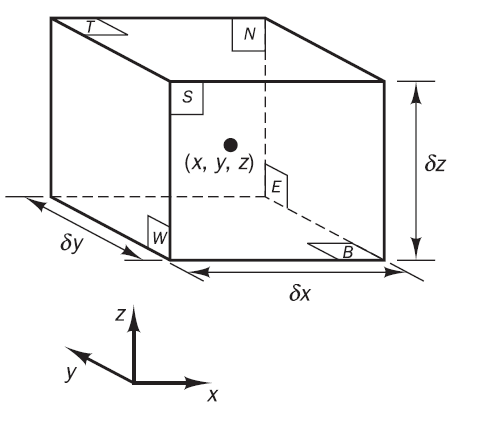
\includegraphics[width =0.3\textwidth]{Images/fig5.png}
	\caption{Fluid element for conservation laws \cite{Versteeg2007}}		
	\label{fig5}
\end{figure}
The six faces are labelled N, S, E, W, T and B, which stands for North, South, East, West, Top and Bottom. The coordinate system is also provided. The centre of the element is located at position \textit{(x,y,x)}. A systematic account of changes in mass, momentum and energy of a fluid element due to fluid flow across its boundaries and, where appropriate, due to the action of sources or sinks inside the element, leads tot the fluid flow equations. \cite{Versteeg2007} \\

In the remainder of this report the fluid element will be treated as an one dimensional element with only East and West faces. Hence, all fluid properties are functions of the $x$-direction, and time only. To prevent ill-chosen confusing notation, the dependence on space and time will not be stated explicitly. For instance, the density of a fluid element at time $t$ is denoted by $\rho$ and the $x$-derivative of, say, the pressure  $p$ at $x$ and time $t$ by $\partial p/\partial x$.

\newpage
\subsection{Conservation of mass} 
The first step in the derivation of the mass conservation equation is to write down a mass balance for the fluid element. In words the mass balance would be:
\setlength{\jot}{0pt}% Inter-equation spacing
\begin{align*}
&&\boxed{
	\begin{aligned}
		&\text{Rate of increase}    &&\text{Net rate of flow} \nonumber \\
		&\text{of mass in fluid} \hspace{0.3cm} =  &&\text{of mass into} \nonumber \\
		&\text{element}  		 	&&\text{fluid element} \nonumber \\
	\end{aligned}
}
\end{align*}

The rate increase of mass in the fluid element is
\begin{align}
	&&\frac{\partial \rho}{\partial t}
	\label{eq1}
\end{align}

The mass flow rate across a face of the element is given by the product of density, area and the velocity component normal to the face. From Figure \ref{fig6} it can be seen that the net rate of flow of mass into the element across its boundaries is given by 
\begin{align}
&&\left(\rho u - \frac{\partial (\rho u)}{\partial x}\frac{1}{2}\partial x\right) -\left( \rho u + \frac{\partial (\rho u)}{\partial x}\frac{1}{2}\partial x\right)
\label{eq2}
\end{align}

Flows which are directed towards the element create an increase of mass, indicated by a positive sign, and the flows leaving the element are given a negative sign.

\begin{figure}[H]
	\centering
	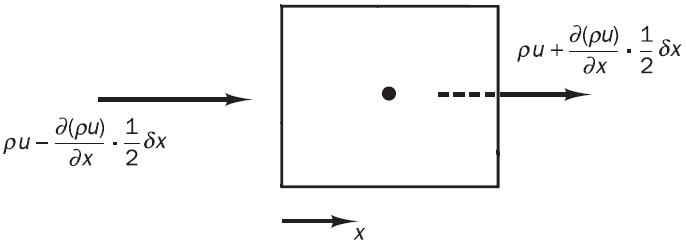
\includegraphics[width =0.45\textwidth]{Images/fig6.png}
	\caption{Mass flows in and out of fluid element \cite{Versteeg2007}}		
	\label{fig6}
\end{figure}

The rate of increase of mass inside the element, Eq. \ref{eq1}, is now equated to the net rate of flow of mass into the element across its faces, Eq. \ref{eq2}. After rearranging all terms to the left hand side of the equals sign and dividing by the element 'volume' $\partial x$ the result is:

\begin{align}
	&& \frac{\partial \rho}{\partial t} + \frac{\partial (\rho u)}{\partial x} =0 
	\label{eq:contbalance}
\end{align}  

Equation \ref{eq:contbalance} is the \textbf{unsteady, one-dimensional mass conservation or continuity equation} at a point in a \textbf{compressible fluid.}.The first term on the left side is the rate of change in time of the density. The second term is called the convective term and  denotes the net flow of mass out of the element across its boundaries. \\
For an \textbf{incompressible fluid} (i.e. a liquid) the density $\rho$ is constant and equation \ref{eq:contbalance} becomes 
\begin{align}
&&	\frac{\partial u}{\partial x} = 0
\end{align}

\newpage
\subsection{The Lagrangian and Eulerian approach}
In the \textbf{Lagrangian approach}, conservation laws state that each property of a particle is a function of the position $x$ of the particle and time $t$. Consider $\phi$ as the value of a property per unit mass. The total or substantive derivative of $\phi$ with respect to time following a fluid particle, written as $D\phi / Dt$, is
\begin{align}
&&	\frac{D \phi}{Dt} = \frac{\partial \phi}{\partial t} + \frac{\partial \phi}{\partial x} \frac{dx}{dt}
\end{align}
A fluid particle follows the flow, so d\textit{x}/d\textit{t} = \textit{u}.\\ 
Hence the substantive derivative of $\phi$ is given by\begin{align}
&&\frac{D \phi}{Dt} = \frac{\partial \phi}{\partial t} + u\frac{\partial \phi}{\partial x} 
\end{align}
$\frac{D \phi}{D t}$ defines rate of change of property $\phi$ per unit mass. \\
Instead of the Lagrangian approach, which is based on tracking the motion and computing rates of change of conserved properties $\phi$ for collections of particles, it is far more common to utilize the Eulerian approach. With the \textbf{Eulerian} approach, equations are developed for collections of fluid elements making up a region fixed in space, for example a region defined by a duct, a pump, a furnace or similar piece of engineering equipment. 
\\ 

As in the case of mass conservation, it is desired to develop equations for rates of change per unit volume. The rate of change of property $\phi$ per unit volume for a fluid particle is given by the product of $D\phi/Dt$ and density $\rho$, hence
\begin{align}
&&\rho\frac{\partial  \phi}{\partial t} = \rho \left(\frac{\partial \phi}{\partial t}  + u\frac{\partial \phi}{\partial x}\right)
\end{align}
\\
The most useful forms of the conservation laws for computational fluid dynamics involve changes of a flow property for a fluid element that is stationary in space. 
\\

The mass conservation equation, Eq. \ref{eq:contbalance}, contains the mass per unit volume (i.e. the density $\rho$) as the conserved quantity. The sum of the rate of change of density in time and the convective term in the mass conservation equation for a fluid element is
\begin{align*}
	&& \frac{\partial \rho}{\partial t} + \frac{\partial (\rho u)}{\partial x}
\end{align*}
The generalisation of these terms for an arbitrary conserved propery is
\begin{align} 
	&& \frac{\partial (\rho \phi)}{\partial t} + \frac{\partial (\rho \phi u)}{\partial x}
	\label{eq3}
\end{align}
Formula \ref{eq3} expresses the rate of change in time of $\phi$ per unit volume plus the net flow of $\phi$ out of the fluid element per unit volume. To illustrate its relation with the substantive derivative of $\phi$ it is rewritten as:
\begin{align}
	&& \frac{\partial(\rho \phi)}{\partial t} + \frac{\partial (\rho \phi u)}{\partial x} &= \rho \left[\frac{\partial \phi}{\partial t} + u \frac{\partial \phi}{\partial x}\right] + \phi \left[\frac{\partial \rho}{\partial t} + \frac{\partial (\rho u)}{\partial x}\right] \nonumber \\ 
	&& &= \rho \frac{D \phi}{D t}
	\label{eq4}
\end{align}
The term $\phi \left[\partial \rho/\partial t +  \partial (\rho u)/\partial x\right]$ is equal to zero by virtue of mass conservation. In words, Equation \ref{eq4} states:
\setlength{\jot}{0pt}% Inter-equation spacing
\begin{align*}
&&\boxed{
	\begin{aligned}
	&\text{Rate of increase}    &&\text{Net rate of flow} &&\text{Rate of increase} \nonumber \\
	&\text{of $\phi$ of fluid} \hspace{0.7cm} +  &&\text{of $\phi$ out of} \hspace{1cm} =  &&\text{of $\phi$ for a} \nonumber \\
	&\text{element}		 	&&\text{fluid element} && \text{fluid particle} \nonumber \\
	\end{aligned}
}
\end{align*}

\subsection{Momentum equation}
Newton's second law states that the rate of change of momentum of a fluid particle equals the sum of the forces on the particle:
\setlength{\jot}{0pt}% Inter-equation spacing
\begin{align*}
&&\boxed{
	\begin{aligned}
	&\text{Rate of increase of}    &&\text{Sum of forces} \nonumber \\
	&\text{momentum of} \hspace{1cm} =  &&\text{on} \nonumber \\
	&\text{fluid particle}	&&\text{fluid particle} \nonumber \\
	\end{aligned}
}
\end{align*}
The rate of increase of x- momentum per unit volume of a fluid particle is give by

\begin{align}
	&&\rho \frac{D u}{Dt}
\end{align}
There are two types of forces on fluid particle:
\begin{itemize}[noitemsep]
	\item surface forces
		\begin{itemize}
			\item pressure forces
			\item viscous forces
			\item gravity force
		\end{itemize}
	\item body forces
		\begin{itemize}
			\item centrifugal force
			\item Coriolis force
			\item electromagnetic forces
		\end{itemize}
\end{itemize}
The surface forces appear in the momentum equation as separate terms and the effect of body forces are included as source terms. The state of stress of a fluid element is defined in terms of the pressure and viscous stress shown in Figure \ref{fig7}. The pressure, a normal stress, is denoted by $p$. Viscous stresses are denoted by $\tau_{xx}$. \\
\begin{figure}[H]
	\centering
	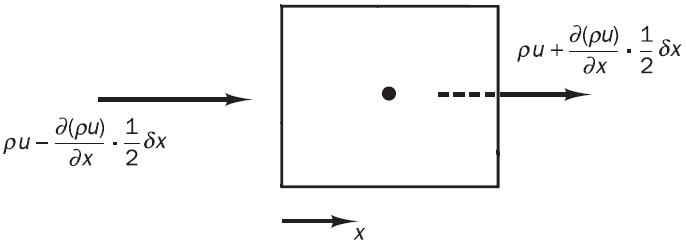
\includegraphics[width =0.45\textwidth]{Images/fig6.png}
	\caption{Stress components in the x-direction \cite{Versteeg2007}}		
	\label{fig7}
\end{figure}
The magnitude of a force resulting from a surface stress is the product of stress and area. Forces aligned with the direction of the x-axis get a positive sign and those in the opposite direction a negative sign. The net force is given by the sum of the force components acting on the fluid element. 

From Figure \ref{fig7} it can be seen that the net force in the \textit{x}-direction is
\begin{align}
	&&\left[\left( p - \frac{\partial p}{\partial x}\frac{1}{2}\partial x\right)- \left( \tau_{xx} - \frac{\partial \tau_{xx}}{\partial x}\frac{1}{2}\partial x\right)\right] + 	\left[-\left( p + \frac{\partial p}{\partial x}\frac{1}{2}\partial x\right)+ \left( \tau_{xx} - \frac{\partial \tau_{xx}}{\partial x}\frac{1}{2}\partial x\right)\right] \nonumber \\ &&= \left(-\frac{\partial p}{\partial x} + \frac{\partial \tau_{xx}}{\partial x}\right) \partial x
\end{align}
The total force per unit volume on the fluid due to the surface stress is equal to 
\begin{align}
	&&\frac{\partial (-p + \tau_{xx})}{\partial x} 
\end{align}
Conservation of momentum Eq. \ref{eq:momentumbalance} is covered by the Navier-Stokes equations
\begin{equation}
\frac{\partial \rho \mathbf{v}}{\partial t} + \nabla \cdot (\rho \mathbf{v} \mathbf{v}) + \nabla \cdot (\boldsymbol{\tau})= -\nabla p + \rho \mathbf{g}
\label{eq:momentumbalance}
\end{equation}

with $\boldsymbol{\tau}$ the stress tensor, p the hydrostatic pressure and $\mathbf{g}$ the acceleration due to gravity. No other body forces than gravity are considered in Eq. \ref{eq:momentumbalance}

For matters of convenience, the conservation of energy in Eq. \ref{eq:enthalpybalance} is written in terms of specific enthalpy $h$
\begin{equation}
\frac{\partial (\rho h)}{\partial t} + \nabla \cdot (\rho \mathbf{v}  h) 
= - \nabla \cdot \mathbf{q} - (\boldsymbol\tau) \colon (\nabla \mathbf{v}) + \frac{D p}{D t}
\label{eq:enthalpybalance}
\end{equation}
where $q$ denotes the heat flux. The second and third term on the right-hand side of Eq. \ref{eq:enthalpybalance} represent enthalpy production due to viscous effects and pressure variations. In Eq. \ref{eq:enthalpybalance}, it is assumed that there are no volumetric heat sources. \\
Note that conservation of energy can also be written in terms of entropy, internal energy or total energy. However, it is of common practice to use the energy equation in its enthalpy form.\\ \\ Finally, conservation of the chemical components is given by transport equations for the species mass fractions Eq.\ref{eq:massbalance}, which are defined as  $Y_k = \rho_k/\rho$ with $\rho_k$ the mass density of species k. \\ By definition:
\begin{equation}
\sum_{k=1}^{N_s} Y_k = 1
\end{equation}

The conservation equations for the species mass fractions is defined as
\begin{equation}
\frac{\partial (\rho Y_k)}{\partial t} + \nabla \cdot \left( \rho \mathbf{v} Y_k\right)
= \nabla \cdot \left( \rho D_k \ \left(\nabla \cdot Y_k\right) \right) + \dot{w_k}
\label{eq:massbalance}
\end{equation}


where $\dot{w_k}$ is the species source term, which will be  discussed later in \hl{Chapter....} and $D_k$ the Diffusion coefficient of species $k$.

\subsection{Equations of state}
The entire problem can be described by the set of differential equations (\ref{eq:contbalance})- (\ref{eq:massbalance}), though the problem is not yet closed. It is completed with two equations of state and a set of constitutive relations. The caloric equation of state for $N_s$ number of species: 
\begin{equation}
h = \sum_{i=1}^{N_s} Y_kh_k
\end{equation}
with 
\begin{equation}
h_k = h_k^{ref} +\int_{T^{ref}}^{T}c_{pk}(T') \ dT'
\label{state1}
\end{equation}
defines the enthalpy $h$ as function of temperature T and species mass fractions assuming that the species are thermally perfect gasses. In Eq \ref{state1} $h_k$, $h_k^{ref}$ and $c_{pk}$ are the specific enthalpy, specific enthalpy of formation at reference temperature $T^{ref}$ and specific heat capacity at constant pressure of species $k$, respectively. The specific heat capacity at constant pressure of the gas mixture is given by
\begin{equation}
c_p = \sum_{i=1}^{N_s} Y_i c_{pi}
\end{equation}
with the species heat capacities $c_{pi}$ well tabulated in polynomial form. In most combustion problems the assumption is made that the gas mixture and its components behave as ideal gasses. Therefore, the thermal equation of state is given by the ideal-gas law:
\begin{equation}
\rho = \frac{p\bar{M}}{RT}
\end{equation}
with R the universal gas constant and $\bar{M}$ the average molar mass. 
Note that for both applications the energy equation is written in terms of enthalpy which is convenient as only the first term of the right hand side remains as a result of the 'Combustion Approximation'.  The energy equation reduces than to Eq\ref{eq:enthalpybalance2}:
\begin{equation}
\frac{\partial (\rho h)}{\partial t} + \nabla \cdot (\rho \boldsymbol{v}  h) 
= - \nabla \cdot \vec{q}
\label{eq:enthalpybalance2}
\end{equation}

\subsection{Constitutive equations}
In order to solve the conservation equations, constitutive equations for $\boldsymbol{\tau},  \ \mathbf{q}$ and $\dot{w_k}$ are necessary. The stress tensor $\boldsymbol{\tau}$ of the gas mixture is assumed to behave the same as the stress tensor for a single-component Newtonian fluid. Using Stokes' assumption the stress tensor can be expressed as:
\begin{equation}
\boldsymbol{{\tau}} = -\mu (\nabla \mathbf{v} +(\mathbf{v})^T) - \frac{2}{3}(\nabla \cdot \mathbf{v})\mathbf{I})
\label{eq:1}
\end{equation} 
where $\mu$ is the dynamic viscosity of the mixture and $\mathbf{I}$ the unit tensor. 
\\

The mixture averaged diffusion coefficient of species $k$ is given by $D_{km}$, where $D_{kj}$ is the diffusivity of species $k$ to $j$:

\begin{equation}
D_{km} = \frac{1 - Y_k}{\sum_{k=1,j\neq k}^{N_s}\frac{X_j}{D_{kj}}}
\end{equation}

\hl{what about self diffusion?}
For the heat flow $\mathbf{q}$ we use the common expression
\begin{equation}
\mathbf{q} = -\lambda \nabla T + \sum_{k=1}^{N_s} \rho D_kY_kh_k
\label{eq:2}
\end{equation}
with $\lambda$ the thermal conductivity of the mixture. Heat transport through conduction and mass diffusion are covered by $\mathbf{q}$ in Eq. \ref{eq:2}. Heat transport due to concentration gradients (Dufour effect) and pressure gradients are neglected

